\chapter{Appendix}
\section{Source alignment}\label{sec:source-alignment}
\begin{figure}
	\centering
		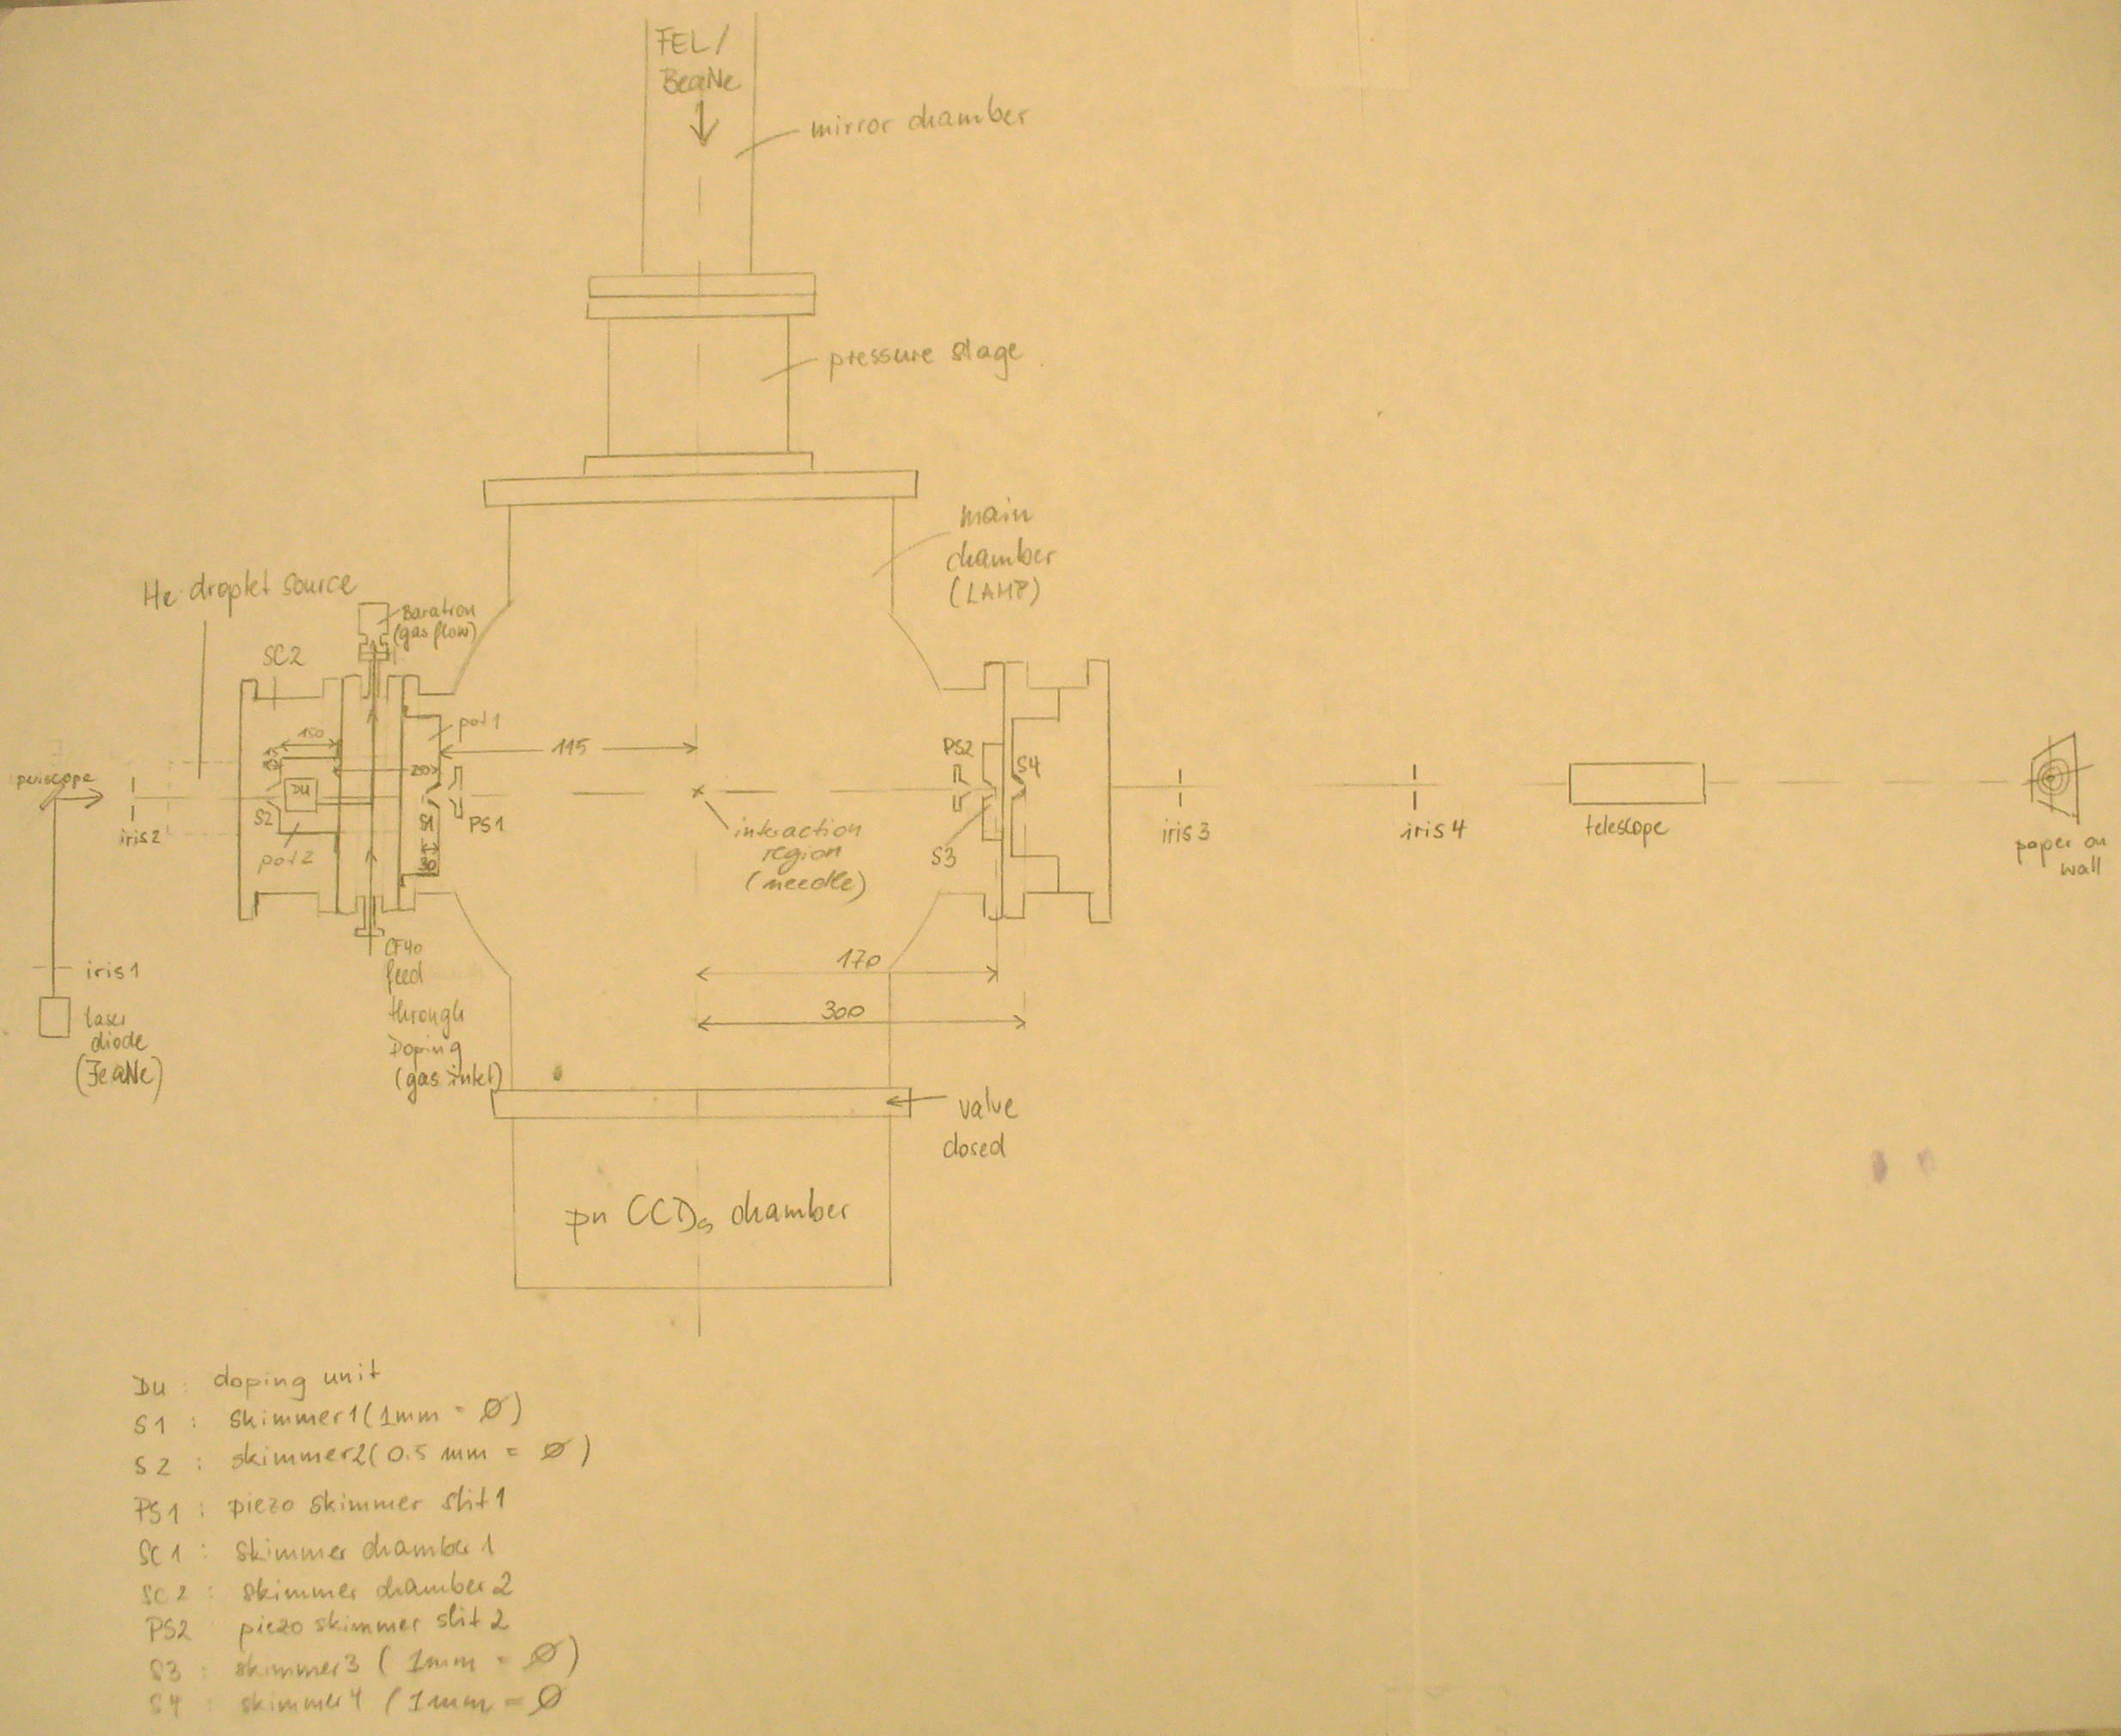
\includegraphics[width=1.00\textwidth]{images/Overview_Setup_Jetalignment.jpg}
	\caption{caption}
	\label{fig:Overview_Setup_Jetalignment}
\end{figure}
%
%
%
\section{Python code psana example}\label{sec:python-example}
Per popular request, a small analysis example is discussed\footnote{Programming languages change their syntax often, it is therefore useful to visit the web-page\\ \url{https://confluence.slac.stanford.edu/display/PSDM/LCLS+Data+Analysis}}. To begin, you should verify that you have a SLAC unix account and a SSH terminal with -Y flag capabilities\footnote{If you have problems with graphics visualization, try the following link\\ \url{https://confluence.slac.stanford.edu/display/PCDS/Remote+Visualization}}. To access the psana computer cluster, see the following commands
\begin{lstlisting}[language=csh,basicstyle=\footnotesize]
	$ ssh -Y USERNAME@pslogin.slac.stanford.edu
	$ ssh -Y psana
	$ source /reg/g/psdm/etc/ana_env.csh
\end{lstlisting}
This logs you into the SLAC psana server and loads the psana framework. Once logged in, make yourself familiar with the following python code ‘psmonLocal.py’. ‘psmonLocal.py’ has been created by Chris O'Grady for demonstration purposes and more information can be found under\\
\url{https://confluence.slac.stanford.edu/display/PSDM/Visualization+Tools}
\lstinputlisting[language=Python,frame=single,basicstyle=\footnotesize]{manuals/psmonLocal.py}
This script demonstrates a pixel detector image (CSpad) and an XY-Plot. Finally, run the script like any python script with
\begin{lstlisting}[language=csh]
	$ python /reg/g/psdm/tutorials/examplePython/psmonLocal.py
\end{lstlisting}
An interesting aspect to the python interaction is the 'TAB' method, where one can code without reading the documentation. Here a user should be on the psana servers and start ipython as follows
\begin{lstlisting}[language=csh,basicstyle=\footnotesize]
	$ ipython
\end{lstlisting}
\begin{lstlisting}[language=Python,basicstyle=\footnotesize]
	$ from psana import *
	$ ds = DataSource('exp=amotut13:run=206')
	$ det = Detector('AmoETOF.0:Acqiris.0')
	$ det.   (NOTE: user hits <TAB> after typing the "." to get list of available methods)
	$ evt = ds.events().next()    (NOTE: getting an event, since the above "Definition" line requires it)
	$ print det.waveform(evt)     (NOTE: calling the "waveform" method as required by the above "Definition" line)
\end{lstlisting}
TBD
%
%
%
\section{Matlab code on spherical integrations}\label{sec:spherical-integration}
Excerpt of the Matlab code that has been used to reduce 2D diffraction images to 1D arrays with the intensity as a function of the scattering vector $\vec{Q}$.
\begin{lstlisting}[language=matlab,frame=single,basicstyle=\footnotesize]
%%% CENTER OF HIT
x_center=xLen/2; % Actually Y-center
y_center=yLen/2; % Actually X-center
for r=(1:1500)
    %looping over points
    for y=(1:yLen)
     for x=(1:xLen)
        %check if in circle
         if (x - x_center)^2 + (y - y_center)^2 < r^2
             %norm
             rnorm(r)=rnorm(r)+1;
             % testing for noise/photons
             if rearpnccd(x,y)>0
              circleSum(r)=circleSum(r)+rearpnccd(x,y);
             end
         elseif (x - x_center)^2 + (y - y_center)^2 == r^2
             %norm
             rnorm(r)=rnorm(r)+(1/2);
             % testing for noise/photons
             if rearpnccd(x,y)>0
               circleSum(r)=circleSum(r)+(rearpnccd(x,y)/2);
             end
         end
     end
    end
    if rnorm(r)==0
        rnorm(r)=1;
    end
    if r==1
        plotSum(r)=circleSum(r)/rnorm(r);
    elseif rnorm(r)-rnorm(r-1)>0
        plotSum(r)=(circleSum(r)-circleSum(r-1))/(rnorm(r)-rnorm(r-1));
    else
        plotSum(r)=0;
    end
end
\end{lstlisting}
%
%
%
\section{Python code on 1D phase-retrieval}\label{sec:1d-phase-retrieval-code}
An excerpt of the python code that has been used to iteratively retrieve the complex fields of the diffraction pattern.
\begin{lstlisting}[language=Python,frame=single,basicstyle=\footnotesize]
# fft
for i in range(1,160):
	print i
	# Fourier Transform to Fourier Space
	fourierSpace = np.fft.fft(realSpaceAdjusted)
	# Get Phase in Fourier Space
	phase = np.exp(np.angle(fourierSpace)*I)
	# Take abslute measurement and multiply with phase
	##fourierSpaceAdjusted = abs(target)*phase
	fourierSpaceAdjusted = abs(np.concatenate((target[0:len(phasedAmplitudes)],fourierSpace[len(phasedAmplitudes):len(phasedAmplitudes)*3],target[len(phasedAmplitudes)*3:len(target)]),axis=0))*phase
	#fourierSpaceAdjusted[fourierSpaceAdjusted[len(phasedAmplitudes):len(phasedAmplitudes)*3] > phasedAmplitudes[len(phasedAmplitudes)-1]] = phasedAmplitudes[len(phasedAmplitudes)-1]
	#print len(fourierSpace)==len(fourierSpaceAdjusted)==len(phase)
	# Calculate Error in Fourier Space
	errorDiffraction = np.append(errorDiffraction,np.std(abs(fourierSpace[0:len(phasedAmplitudes)]) - abs(target[0:len(phasedAmplitudes)])))
	###
	# Fourier Transform to Real Space
	realSpace = np.fft.ifft(fourierSpaceAdjusted)
	realSpaceAdjusted = realSpace.real
	#print len(realSpace)==len(realSpaceAdjusted)
	# Set values to zero where object not expected
	#realSpaceAdjusted[30:len(realSpaceAdjusted)-30] = np.zeros(len(realSpaceAdjusted)-60)
	realSpaceAdjusted[realSpaceAdjusted < 0] = 0
	# Claculate error of Support
	errorSupport = np.append(errorSupport,np.sum(abs(np.fft.ifftshift(realSpace)[0:len(realSpace)/2 - 30])))
	#print errorSupport
\end{lstlisting}
%
%
%
\section{Python code on combining detectors}\label{sec:combination-of-detectors-code}
Python code that has been used to combine pnCCD detectors.
\lstinputlisting[language=Python,frame=single,basicstyle=\footnotesize]{manuals/combination.py}
%
%
%